\documentclass{beamer}
% Use DS9 global theme
\usepackage{../../../shared/templates/ds9_theme}

\title[Work \& Energy]{PHYS11 CH9: Work, Energy, and Energy Conservation}
\subtitle{From Work to Energy Conservation}
\author[Mr. Gullo]{Mr. Gullo}
\date[Feb 2025]{February, 2025}


\begin{document}

\frame{\titlepage}

\begin{frame}
\frametitle{Chapter Sections}
\tableofcontents
\end{frame}

\section{9.1 Work, Power, and the Work-Energy Theorem}

\begin{frame}
\frametitle{9.1 Learning Objectives}
By the end of this section, you will be able to:
\begin{itemize}
\item Describe and apply the work-energy theorem
\item Describe and calculate work and power
\end{itemize}
\end{frame}

\begin{frame}
\frametitle{9.1 Understanding Work}
\begin{block}{Work Definition}
Work = Force × Distance (in direction of force)
$$W = F \cdot d$$
\end{block}

\begin{block}{Key Points About Work}
\begin{itemize}
\item Work is done only when force causes displacement
\item Force must be parallel to displacement
\item Work can be positive or negative:
 \begin{itemize}
 \item Positive: Force in same direction as motion
 \item Negative: Force opposing motion
 \end{itemize}
\item No work is done when:
 \begin{itemize}
 \item Force is perpendicular to motion
 \item No displacement occurs
 \end{itemize}
\end{itemize}
\end{block}
\end{frame}

\begin{frame}
\frametitle{9.1 Work and Force Relationships}
\begin{block}{Force and Weight}
$$F = w = mg$$
Where:
\begin{itemize}
\item $F$ = Force (N)
\item $w$ = Weight (N)
\item $m$ = Mass (kg)
\item $g$ = Gravitational acceleration (9.8 m/s²)
\end{itemize}
\end{block}
\end{frame}

\begin{frame}
\frametitle{Work and Changes in Gravitational Potential Energy}
\begin{block}{Work and $\Delta PE_g$ Relationship}
$$W = \Delta PE_g = mg\Delta h = mg(h_2 - h_1)$$
Where:
\begin{itemize}
\item $W$ = Work done (J)
\item $\Delta PE_g$ = Change in gravitational potential energy (J)
\item $m$ = Mass of object (kg)
\item $g$ = Gravitational acceleration (9.8 m/s²)
\item $h_2$ = Final height (m)
\item $h_1$ = Initial height (m)
\item $\Delta h$ = Change in height = $h_2 - h_1$ (m)
\end{itemize}
\end{block}
\end{frame}

\begin{frame}
\begin{alertblock}{Important Note}
\begin{itemize}
\item Positive work ($\Delta h > 0$): Lifting object against gravity
\item Negative work ($\Delta h < 0$): Object falling with gravity
\item Work done against gravity equals the change in gravitational potential energy of the object
\end{itemize}
\end{alertblock}
\end{frame}

\begin{frame}
\frametitle{9.1 Work-Energy Theorem}
\begin{block}{Work-Energy Theorem}
$$W = \Delta KE = \frac{1}{2}mv_2^2 - \frac{1}{2}mv_1^2$$
\end{block}

\begin{block}{Components}
Where:
\begin{itemize}
\item $W$ = Net work done on object (J)
\item $\Delta KE$ = Change in kinetic energy (J)
\item $m$ = Mass of object (kg)
\item $v_1$ = Initial velocity (m/s)
\item $v_2$ = Final velocity (m/s)
\end{itemize}
\end{block}
\end{frame}

\begin{frame}
\begin{alertblock}{Key Concept}
The net work done on an object equals its change in kinetic energy. This means:
\begin{itemize}
\item Positive work increases kinetic energy ($v_2 > v_1$)
\item Negative work decreases kinetic energy ($v_2 < v_1$)
\end{itemize}
\end{alertblock}
\end{frame}

\begin{frame}
\frametitle{9.1 Power - Rate of Work}
\begin{block}{Power Definition}
$$P = \frac{W}{t}$$
Rate at which work is done or energy is transferred
\end{block}
\end{frame}

\begin{frame}
\begin{block}{Power Relationships}
Alternative forms:
\begin{align*}
P &= \frac{W}{t} = \frac{Fd}{t} = F\cdot v \\[1em]
P &= \frac{\Delta E}{t}
\end{align*}
Where:
\begin{itemize}
\item $P$ = Power (watts, W)
\item $W$ = Work done (joules, J)
\item $t$ = Time interval (seconds, s)
\item $F$ = Force (newtons, N)
\item $v$ = Velocity (m/s)
\item $\Delta E$ = Energy change (J)
\end{itemize}
\end{block}

\begin{exampleblock}{Real-World Applications}
\begin{itemize}
\item Engine power ratings
\item Electrical appliance ratings
\item Human power output in athletics
\end{itemize}
\end{exampleblock}
\end{frame}

\begin{frame}
\frametitle{9.1 Example: Calculating Work}
Problem: Calculate the work done lifting a 2.0 kg book 1.5 m vertically.
\begin{block}{Solution}
\begin{enumerate}
\item Force needed = weight = mg = (2.0 kg)(9.8 m/s²) = 19.6 N
\item Distance = 1.5 m
\item Work = F × d = 19.6 N × 1.5 m = 29.4 J
\end{enumerate}
\end{block}
\end{frame}
\begin{frame}
\frametitle{Units of Work}
\begin{block}{Work = Force × Distance}
$$W = F \cdot d$$
\end{block}

\begin{block}{SI Units}
\begin{itemize}
\item Force (F): Newtons (N)
\item Distance (d): meters (m)
\item Work (W): Newton-meters (N⋅m) = Joules (J)
\end{itemize}
\end{block}

\begin{block}{Unit Analysis}
$$1 \text{ Joule} = 1 \text{ N} \cdot 1 \text{ m} = 1 \text{ kg}\cdot\frac{\text{m}}{\text{s}^2} \cdot \text{m} = 1 \text{ kg}\cdot\frac{\text{m}^2}{\text{s}^2}$$
\end{block}
\end{frame}

\begin{frame}
\frametitle{Units of Power}
\begin{block}{Power = Work ÷ Time}
$$P = \frac{W}{t}$$
\end{block}

\begin{block}{SI Units}
\begin{itemize}
\item Work (W): Joules (J)
\item Time (t): seconds (s)
\item Power (P): Joules per second (J/s) = Watts (W)
\end{itemize}
\end{block}

\begin{block}{Common Power Units}
\begin{itemize}
\item 1 kilowatt (kW) = 1,000 watts
\item 1 horsepower (hp) ≈ 746 watts
\item 1 kilowatt-hour (kWh) = power × time = 3,600,000 joules
\end{itemize}
\end{block}
\end{frame}

\begin{frame}
\frametitle{Units in Energy Equations}
\begin{block}{Kinetic Energy}
$$KE = \frac{1}{2}mv^2$$
Units: $\text{kg} \cdot (\frac{\text{m}}{\text{s}})^2 = \text{kg}\cdot\frac{\text{m}^2}{\text{s}^2} = \text{Joules}$
\end{block}

\begin{block}{Gravitational Potential Energy}
$$PE = mgh$$
Units: $\text{kg} \cdot \frac{\text{m}}{\text{s}^2} \cdot \text{m} = \text{kg}\cdot\frac{\text{m}^2}{\text{s}^2} = \text{Joules}$
\end{block}

\begin{exampleblock}{Unit Consistency}
All forms of energy (KE, PE, Work) are measured in Joules, allowing direct comparison and conversion between different forms of energy.
\end{exampleblock}
\end{frame}

\begin{frame}
\begin{figure}
    \centering
    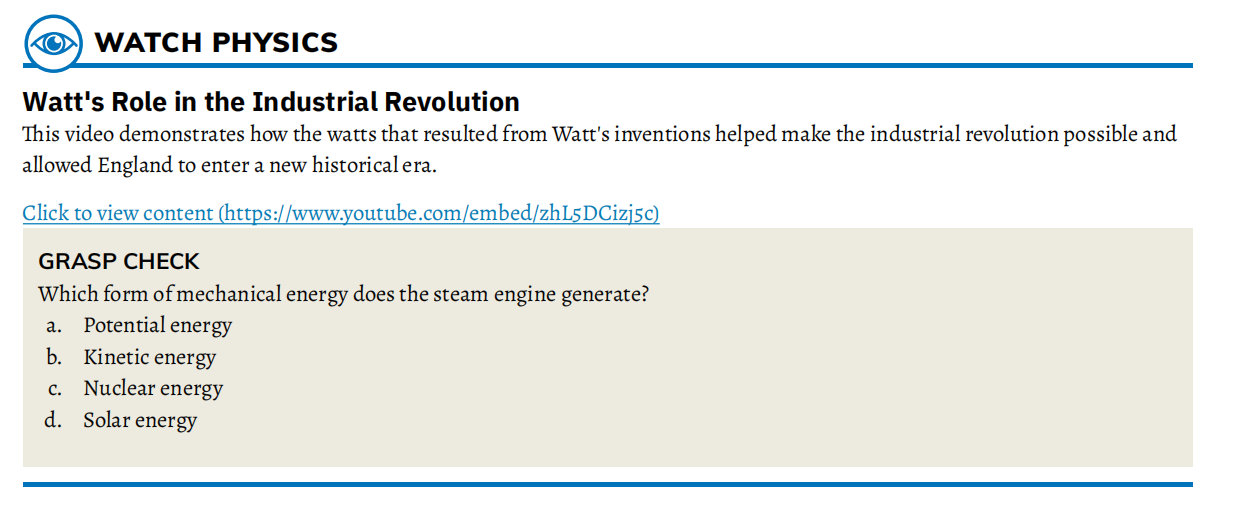
\includegraphics[width=1\linewidth]{phys11-energy-watts-industrial-revolution.png}
\end{figure}
\end{frame}

\section{9.2 Mechanical Energy and Conservation of Energy}

\begin{frame}
\frametitle{9.2 Learning Objectives}
By the end of this section, you will be able to:
\begin{itemize}
\item Explain the law of conservation of energy
\item Perform calculations with mechanical energy
\item Apply conservation of energy principles
\end{itemize}
\end{frame}

\begin{frame}
\frametitle{9.2 Types of Mechanical Energy}
\begin{block}{Kinetic Energy (Energy of Motion)}
$$KE = \frac{1}{2}mv^2$$
\end{block}

\begin{block}{Gravitational Potential Energy}
$$PE = mgh$$
\end{block}
\end{frame}

\begin{frame}
\frametitle{9.2 Conservation of Mechanical Energy}
\begin{block}{Energy Conservation Equation}
$$E_{total} = E_{mechanical} = KE + PE = \text{constant}$$
$$\therefore KE_1 + PE_1 = KE_2 + PE_2$$
\end{block}

\begin{alertblock}{What This Means}
In a closed system with no friction:
\begin{itemize}
\item Initial Energy = Final Energy
\item $\frac{1}{2}mv_1^2 + mgh_1 = \frac{1}{2}mv_2^2 + mgh_2$
\end{itemize}
\end{alertblock}
\end{frame}

\begin{frame}
\begin{figure}
    \centering
    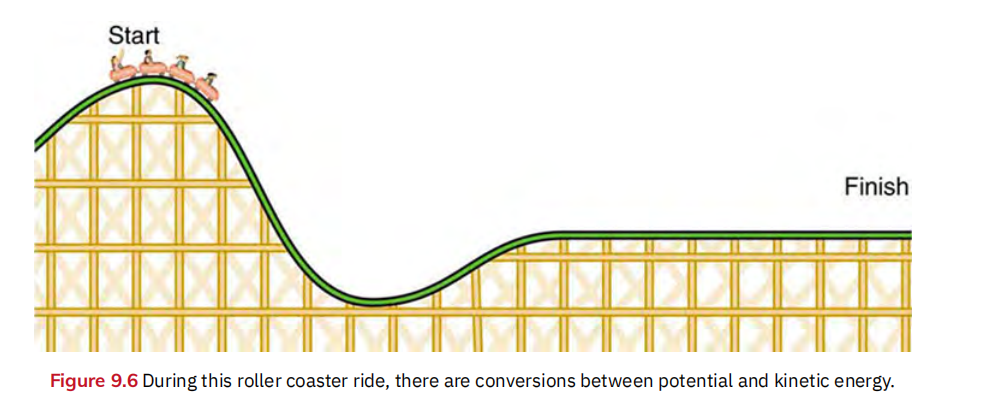
\includegraphics[width=0.5\linewidth]{phys11-energy-conservation-roller-coaster.png}
\end{figure}
\begin{block}{Energy Transformations}
\begin{center}
\begin{tabular}{c c c}
\textbf{State 1} & $\rightarrow$ & \textbf{State 2} \\
\hline
High PE, Low KE & $\rightarrow$ & Low PE, High KE \\
(Top of hill) & & (Bottom of hill) \\[1em]
Low PE, High KE & $\rightarrow$ & High PE, Low KE \\
(Bottom of hill) & & (Top of hill)
\end{tabular}
\end{center}
\end{block}
\end{frame}

\begin{frame}
\frametitle{9.2 Energy Conservation Examples}
\begin{block}{Example: Roller Coaster}
\begin{itemize}
\item At top: High PE, Low KE
 $$PE_{max} = mgh, \quad KE \approx 0$$
\item At bottom: Low PE, High KE
 $$PE \approx 0, \quad KE_{max} = \frac{1}{2}mv^2$$
\item Total Energy stays constant:
 $$mgh = \frac{1}{2}mv^2$$
\end{itemize}
\end{block}
\end{frame}

\begin{frame}
\begin{exampleblock}{Key Points}
\begin{itemize}
\item Energy is never created or destroyed
\item Energy only transforms from one form to another
\item In real systems, some mechanical energy converts to heat due to friction
\item Total system energy always remains constant
\end{itemize}
\end{exampleblock}
\end{frame}

\begin{frame}
\frametitle{9.2 Example: Energy Conservation}
A roller coaster car (500 kg) starts from rest at height 40 m. What is its speed at height 15 m?
\begin{figure}
    \centering
    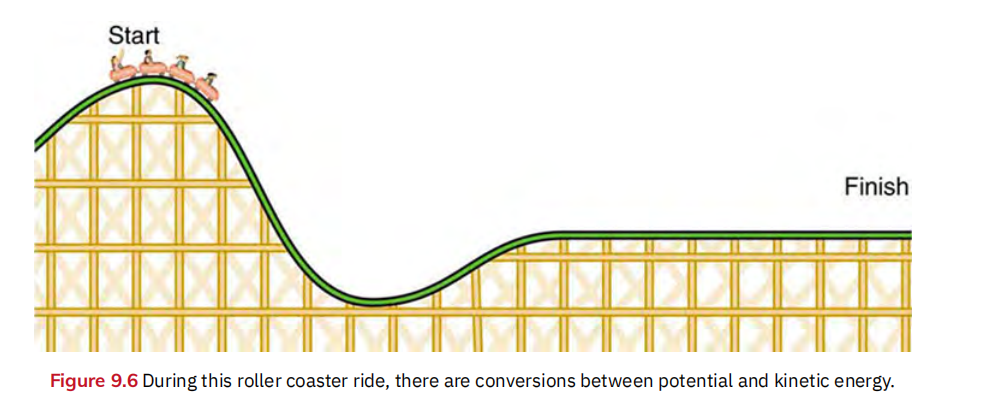
\includegraphics[width=0.5\linewidth]{phys11-energy-conservation-roller-coaster.png}
\end{figure}

\end{frame}


\begin{frame}
\begin{block}{Solution Steps}
\begin{enumerate}
\item Initial PE = mgh₁ = (500)(9.8)(40) = 196,000 J
\item Final PE = mgh₂ = (500)(9.8)(15) = 73,500 J
\item Conservation: PE₁ = PE₂ + KE₂
\item 196,000 = 73,500 + ½(500)v²
\item Solve for v
\end{enumerate}
\end{block}
\end{frame}

\section{9.3 Simple Machines}

\begin{frame}
\frametitle{9.3 Learning Objectives}
By the end of this section, you will be able to:
\begin{itemize}
\item Describe simple and complex machines
\item Calculate mechanical advantage and efficiency
\end{itemize}
\end{frame}

\begin{frame}
\frametitle{9.3 Simple Machines: Basic Mechanical Advantage}
\begin{block}{General Ideal Mechanical Advantage (IMA)}
$$IMA = \frac{F_r}{F_e} = \frac{d_e}{d_r}$$
Where:
\begin{itemize}
\item $F_r$ = Resistance force (output force)
\item $F_e$ = Effort force (input force)
\item $d_e$ = Distance effort moves
\item $d_r$ = Distance resistance moves
\end{itemize}
\end{block}
\end{frame}

\begin{frame}
\frametitle{9.3 Simple Machines: Levers and Wheel-Axle}
\begin{block}{Lever}
$$IMA = \frac{L_e}{L_r}$$
Where:
\begin{itemize}
\item $L_e$ = Length of effort arm
\item $L_r$ = Length of resistance arm
\end{itemize}
\end{block}

\begin{figure}
    \centering
    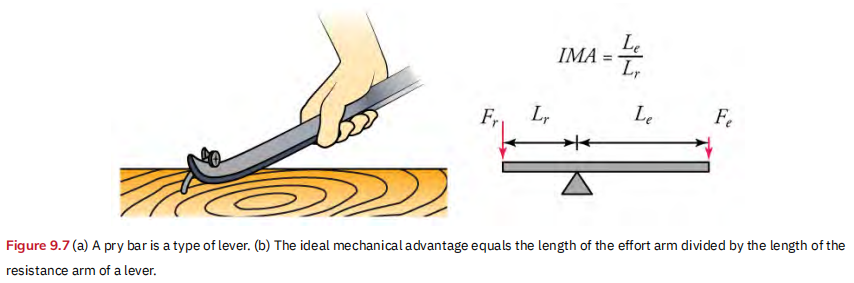
\includegraphics[width=0.75\linewidth]{phys11-machines-lever-diagram.png}
\end{figure}
\end{frame}

\begin{frame}
\begin{block}{Wheel and Axle}
$$IMA = \frac{R}{r}$$
Where:
\begin{itemize}
\item $R$ = Radius of wheel
\item $r$ = Radius of axle
\end{itemize}
\end{block}
\begin{figure}
    \centering
    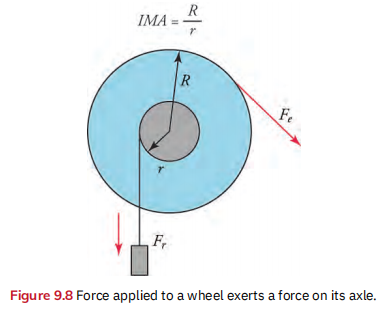
\includegraphics[width=0.5\linewidth]{phys11-machines-axle-diagram.png}
\end{figure}
\end{frame}

\begin{frame}
\frametitle{9.3 Simple Machines: Inclined Plane and Wedge}
\begin{block}{Inclined Plane}
$$IMA = \frac{L}{h}$$
Where:
\begin{itemize}
\item $L$ = Length of slope
\item $h$ = Vertical height
\end{itemize}
\end{block}
\begin{figure}
    \centering
    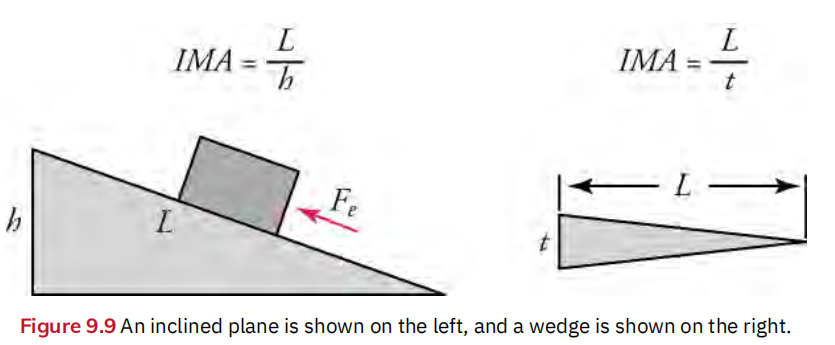
\includegraphics[width=0.5\linewidth]{InclinePlane.png}
\end{figure}

\end{frame}

\begin{frame}


\begin{block}{Wedge}
$$IMA = \frac{L}{t}$$
Where:
\begin{itemize}
\item $L$ = Length of wedge
\item $t$ = Thickness of wedge
\end{itemize}
\end{block}
\begin{figure}
    \centering
    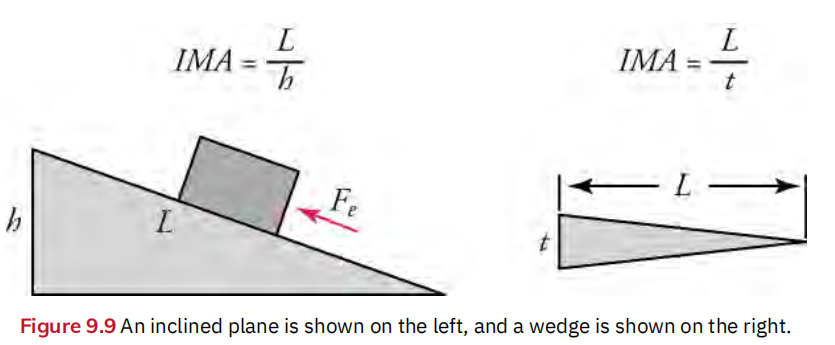
\includegraphics[width=0.5\linewidth]{InclinePlane.png}
\end{figure}
\end{frame}

\begin{frame}
\frametitle{9.3 Simple Machines: Pulley and Screw}
\begin{block}{Pulley}
$$IMA = N$$
Where:
\begin{itemize}
\item $N$ = Number of rope sections supporting the load
\end{itemize}
\end{block}
\begin{figure}
    \centering
    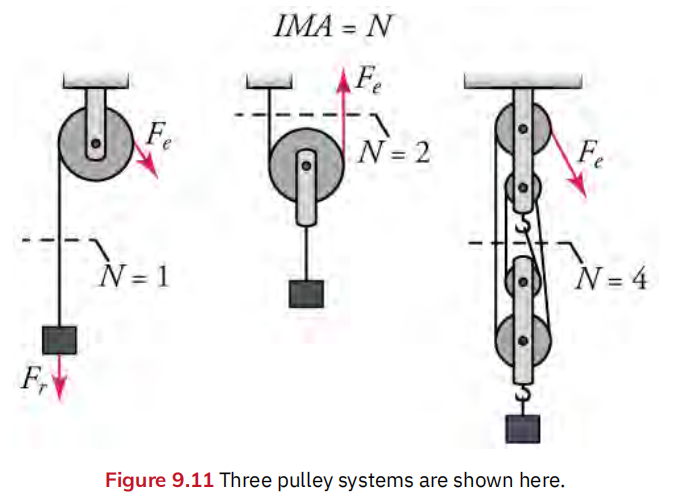
\includegraphics[width=0.5\linewidth]{Pulley.png}
\end{figure}
\end{frame}

\begin{frame}
\begin{block}{Screw}
$$IMA = \frac{2\pi L}{P}$$
Where:
\begin{itemize}
\item $L$ = Length of effort arm
\item $P$ = Pitch (distance between threads)
\item $2\pi$ = Circumference factor
\end{itemize}
\end{block}
\begin{figure}
    \centering
    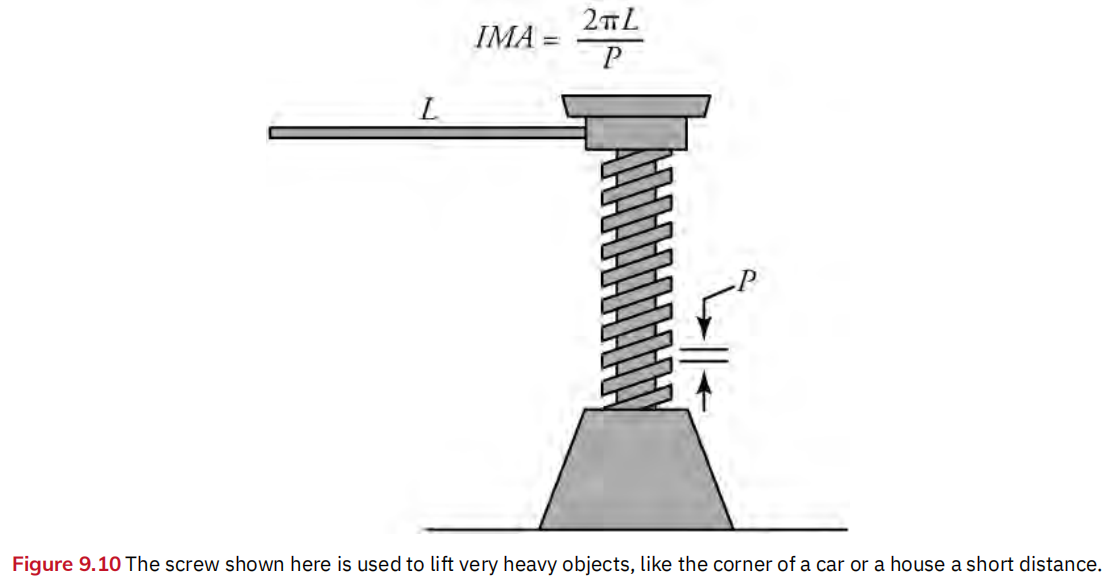
\includegraphics[width=0.5\linewidth]{phys11-machines-screw-diagram.png}
\end{figure}
\end{frame}

\begin{frame}
\frametitle{9.3 Work Input and Output}
\begin{block}{Input Work}
$$W_i = F_id_i$$
Where:
\begin{itemize}
\item $W_i$ = Work input (energy put into machine)
\item $F_i$ = Input force (effort force)
\item $d_i$ = Input distance (distance effort moves)
\end{itemize}
\end{block}

\begin{block}{Output Work}
$$W_o = F_od_o$$
Where:
\begin{itemize}
\item $W_o$ = Work output (useful work done by machine)
\item $F_o$ = Output force (resistance force)
\item $d_o$ = Output distance (distance load moves)
\end{itemize}
\end{block}
\end{frame}

\begin{frame}
\frametitle{9.3 Machine Efficiency}
\begin{block}{Efficiency Formula}
$$\text{Efficiency} = \frac{W_o}{W_i} \times 100\%$$
\end{block}

\begin{block}{Important Points}
\begin{itemize}
\item Efficiency is always less than 100% in real machines
\item Energy is lost to:
 \begin{itemize}
 \item Friction between moving parts
 \item Heat generation
 \item Sound production
 \end{itemize}
\item Higher efficiency means less energy waste
\item Efficiency can be improved through:
 \begin{itemize}
 \item Better lubrication
 \item Smoother surfaces
 \item Proper maintenance
 \end{itemize}
\end{itemize}
\end{block}
\end{frame}

\begin{frame}
\frametitle{Chapter Summary}
\begin{itemize}
\item \textbf{9.1 Work and Power}
  \begin{itemize}
  \item Work is force times distance
  \item Power is rate of doing work
  \end{itemize}
\item \textbf{9.2 Energy Conservation}
  \begin{itemize}
  \item Energy transforms between forms
  \item Total energy is conserved
  \end{itemize}
\item \textbf{9.3 Simple Machines}
  \begin{itemize}
  \item Machines trade force for distance
  \item Efficiency measures useful work output
  \end{itemize}
\end{itemize}
\end{frame}

\end{document}